\chapter{Functional Requirements}
\section{Useage Model}
\scalebox{0.6}{
	
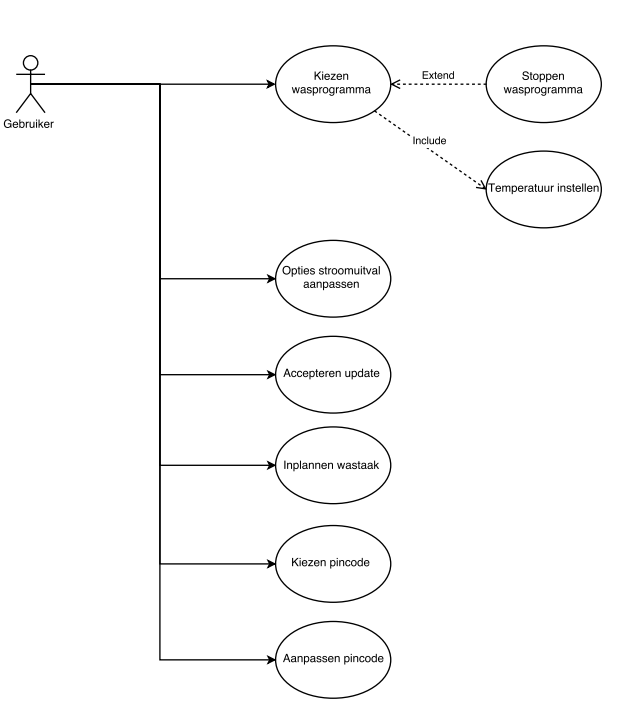
\includegraphics{usage_1.png}
}
\newpage
\scalebox{0.6}{
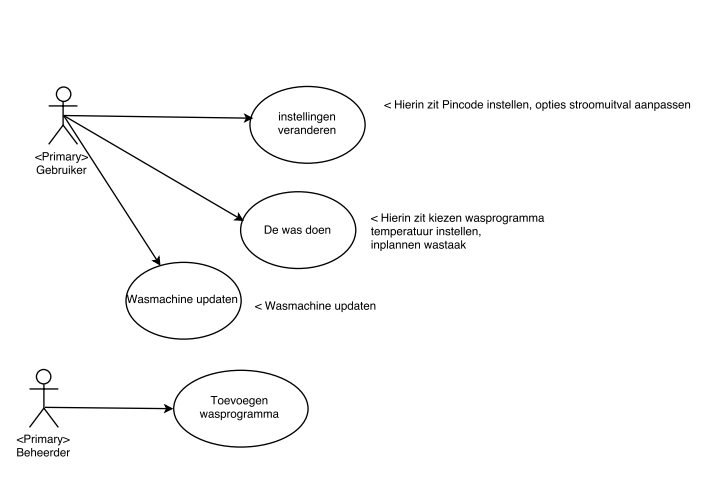
\includegraphics{usage_2.png}
	
}
\section{Inleiding}
In dit hoofdstuk zullen de use-cases worden beschreven.
Wanneer er wordt gerefereerd naar een "gebruiker" dan wordt hiermee de klant bedoelt die de wasmachine gekocht heeft en deze gebruikt om de was mee te doen.
Een "beheerder" is iemand die werkt voor het bedrijf die wasmachine's levert en beheert.
\newpage
\section{Use Case Beschrijvingen}
\subsection{Kiezen Wasprogramma}
\begin{center}
  \begin{tabular}{ | p{4cm} | p{8.5cm} | }    \hline
    Doel & Het kiezen van een wasprogramma om deze te starten. \\ \hline
    Pre-condities & De gebruiker is ingelogd op de webinterface. \\ \hline
    Post-condities & De wasmachine is gestopt met wassen en het water is weg gepompt. \\ \hline
    Uitzonderingen & De gebruiker klikt op de knop "Stop". Hierdoor wordt de huidige wastaak stopgezet. De wasmachine pompt het water weg. \\
    \hline
  \end{tabular}
\end{center}

\subsection{Temperatuur instellen}
\begin{center}
  \begin{tabular}{ | p{4cm} | p{8.5cm} | }    \hline
    Doel & Het aanpassen van de temperatuur van het huidige wasprogramma. \\ \hline
    Pre-condities & De gebruiker is ingelogd op de webinterface door middel van een pincode en heeft een wasprogramma gekozen. \\ \hline
    Post-condities & De wasmachine is een wastaak begonnen met de aangegeven temperatuur. \\ \hline
    Uitzonderingen &  \\
    \hline
  \end{tabular}
\end{center}

\subsection{Opties stroomuitval aanpassen}
\begin{center}
  \begin{tabular}{ | p{4cm} | p{8.5cm} | }    \hline
    Doel & Het aanpassen van de instellingen voor het beveiligen tegen stroomuitval. \\ \hline
    Pre-condities & De gebruiker is ingelogd op de webinterface door middel van een pincode. \\ \hline
    Post-condities & De instelling voor het beveiligen tegen stroomuitval zijn opgeslagen. \\ \hline
    Uitzonderingen &  \\
    \hline
  \end{tabular}
\end{center}

\subsection{Accepteren update}
\begin{center}
  \begin{tabular}{ | p{4cm} | p{8.5cm} | }    \hline
    Doel & Het accepteren van een nieuw wasprogramma door middel van een automatische update. \\ \hline
    Pre-condities & De gebruiker is ingelogd op de webinterface door middel van een pincode. \\ \hline
    Post-condities & Een nieuw wasprogramma is toegevoegd aan de lijst van wasprogramma's. \\ \hline
    Uitzonderingen &  \\
    \hline
  \end{tabular}
\end{center}

\subsection{Inplannen wastaak}
\begin{center}
  \begin{tabular}{ | p{4cm} | p{8.5cm} | }    \hline
    Doel & Het automatisch laten uitvoeren van een wastaak nadat een bepaalde tijd verstreken is. \\ \hline
    Pre-condities & De gebruiker is ingelogd op de webinterface door middel van een pincode. \\ \hline
    Post-condities & De wasmachine is na een aangegeven periode begonnen met het uitvoeren van de aangegeven wastaak. \\ \hline
    Uitzonderingen &  \\
    \hline
  \end{tabular}
\end{center}

\subsection{Kiezen pincode}
\begin{center}
  \begin{tabular}{ | p{4cm} | p{8.5cm} | }    \hline
    \hline
    Doel & De gebruiker een pincode laten kiezen voor het inloggen op de webinterface. \\ \hline
    Pre-condities & Geen pre-conditie. \\ \hline
    Post-condities & De pincode is ingesteld als login pin voor de webinterface. \\ \hline
    Uitzonderingen &  \\
    \hline
  \end{tabular}
\end{center}

\subsection{Aanpassen pincode}
\begin{center}
  \begin{tabular}{ | p{4cm} | p{8.5cm} | }    \hline
    Doel & De gebruiker de huidige pincode laten aanpassen. \\ \hline
    Pre-condities & De gebruiker is ingelogd op de webinterface. \\ \hline
    Post-condities & De huidige pincode is vervangen door de nieuwe pincode als login. \\ \hline
	Uitzonderingen &  \\
    \hline
  \end{tabular}
\end{center}

\section{Activity Diagrams}
\scalebox{0.6}{
	
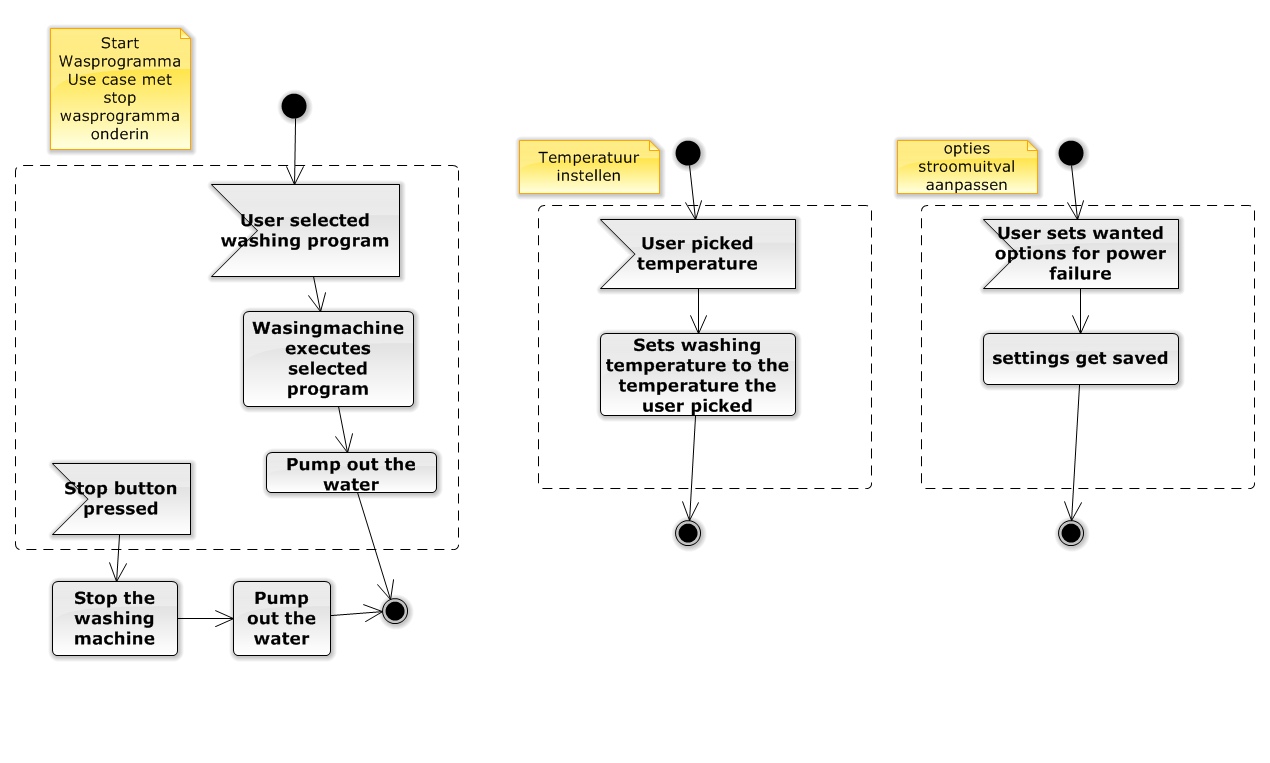
\includegraphics{activity_1.png}
}